%----------------------------------------------------------------------------------------
%	PACKAGES AND OTHER DOCUMENT CONFIGURATIONS
%----------------------------------------------------------------------------------------

\documentclass{article}

\usepackage{fancyhdr} % Required for custom headers
\usepackage{lastpage} % Required to determine the last page for the footer
\usepackage{extramarks} % Required for headers and footers
\usepackage{graphicx} % Required to insert images
\usepackage{pdflscape} % Allow us to make certain pages in landscape orientation
\usepackage{amsmath} % Allow multiple line equations
\usepackage{amssymb}
\usepackage{scrextend}
\usepackage{xcolor}
\usepackage{listings}

\definecolor{mGreen}{rgb}{0,0.6,0}
\definecolor{mGray}{rgb}{0.5,0.5,0.5}
\definecolor{mPurple}{rgb}{0.58,0,0.82}
\definecolor{backgroundColour}{rgb}{0.95,0.95,0.92}

\lstdefinestyle{CStyle}{
    backgroundcolor=\color{backgroundColour},   
    commentstyle=\color{mGreen},
    keywordstyle=\color{magenta},
    numberstyle=\tiny\color{mGray},
    stringstyle=\color{mPurple},
    basicstyle=\footnotesize,
    breakatwhitespace=false,         
    breaklines=true,                 
    captionpos=b,                    
    keepspaces=true,                 
    numbers=none,                   
    numbersep=5pt,                  
    showspaces=false,                
    showstringspaces=false,
    showtabs=false,                  
    tabsize=2,
    language=C
}

% Margins
\topmargin=-0.45in
\evensidemargin=0in
\oddsidemargin=0in
\textwidth=6.5in
\textheight=9.0in
\headsep=0.25in 

\linespread{1.1} % Line spacing

% Set up the header and footer
\pagestyle{fancy}
\chead{\Title} % Top center header
\rhead{\firstxmark} % Top right header
\lfoot{\lastxmark} % Bottom left footer
\cfoot{} % Bottom center footer
\rfoot{Page\ \thepage\ of\ \pageref{LastPage}} % Bottom right footer
\renewcommand\headrulewidth{0.4pt} % Size of the header rule
\renewcommand\footrulewidth{0.4pt} % Size of the footer rule

\setlength\parindent{0pt} % Removes all indentation from paragraphs

%----------------------------------------------------------------------------------------
%	DOCUMENT STRUCTURE COMMANDS
%----------------------------------------------------------------------------------------

\setcounter{secnumdepth}{0} % Removes default section numbers
   
%----------------------------------------------------------------------------------------
%	NAME AND CLASS SECTION
%----------------------------------------------------------------------------------------

\newcommand{\Title}{Assignment 1} % Assignment title
\newcommand{\DueDate}{21 April 2018} % Due date
\newcommand{\Class}{CAB202 - Microprocessors and Digital Systems} % Course/class
\newcommand{\AuthorName}{Pedro Alves (n9424342)}

%----------------------------------------------------------------------------------------
%	TITLE PAGE
%----------------------------------------------------------------------------------------

\title{
\vspace{2in}
\textmd{\huge\textbf{\Class}}\\
\textmd{{\Title}}\\
\vspace{3in}
\textmd{{\AuthorName}}\\
}

%----------------------------------------------------------------------------------------

\begin{document}

\maketitle
\clearpage

%----------------------------------------------------------------------------------------
%	TABLE OF CONTENTS
%----------------------------------------------------------------------------------------

%\setcounter{tocdepth}{1} % Uncomment this line if you don't want subsections listed in the ToC

\newpage
\tableofcontents
\newpage

%----------------------------------------------------------------------------------------
%	EXECUTIVE SUMMARY
%----------------------------------------------------------------------------------------
\section{Executive Summary}

\clearpage

%----------------------------------------------------------------------------------------
%	PROGRAM OVERVIEW
%----------------------------------------------------------------------------------------
\section{Program Overview}
Things to talk about
\newline
change\_state
\clearpage

%----------------------------------------------------------------------------------------
%	SPLASH SCREEN
%----------------------------------------------------------------------------------------
\section{Splash Screen}
 The splash screen is the first screen the player sees when they start the game. It provides basic information about the game and will change to the main game screen when the player presses any key.

\subsection*{Functions}
\begin{lstlisting}[style=CStyle]
	// main.c
	void update_start_screen();
\end{lstlisting}
Called every tick of the main game loop. Will change the game's state to \emph{GAME\_SCREEN} if there is any key in the input buffer. Since the \emph{change\_state()} function already purges the input buffer, we do not have to worry about the game skipping straight to the \emph{GAME\_SCREEN}.
\begin{lstlisting}[style=CStyle]
	// main.c
	void draw_start_screen();
\end{lstlisting}
Calculates the x and y coordinates of each string to be shown based on the dimensions of the screen. Will then call \emph{draw\_string()} and \emph{draw\_center\_text()} multiple times to add the strings to the desired location.
\begin{lstlisting}[style=CStyle]
	// main.c
	void draw_center_text(char * text, int y);
\end{lstlisting}
Calculates what x coordinate is required in order to have the text appear at the middle of the screen. Then calls \emph{draw\_string()} to print the text. 
\newline

\subsection*{Testing}
Testing that the splash screen shows up when the game is started.
\begin{figure}[h]
	\begin{center}
	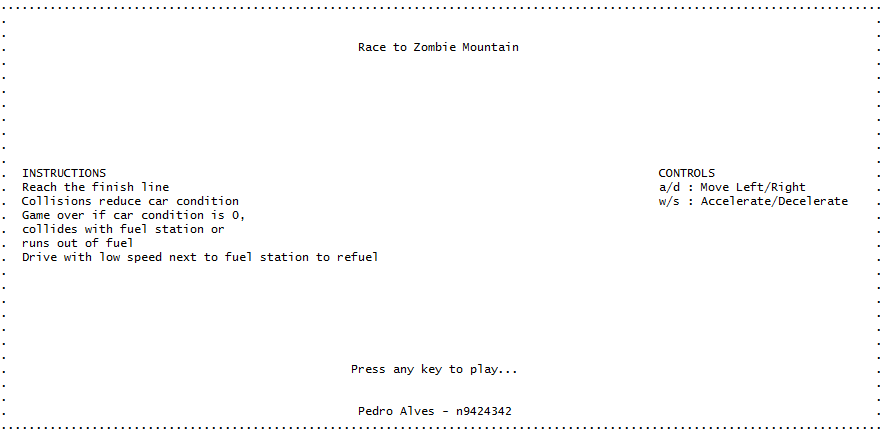
\includegraphics[width=1\textwidth]{images/splash_screen}
	\caption{The splash screen when the player starts the game}
	\label{fig:splash_screen} 
	\end{center}
\end{figure}

\clearpage

%----------------------------------------------------------------------------------------
%	BORDER
%----------------------------------------------------------------------------------------
\section{Border}
The border is simply a rectangle that is drawn on the edge of the terminal. It supports every terminal size.
\newline
The \emph{draw\_borders()} functon is the last one called before \emph{show\_screen()} in the draw step of the game loop. This ensures that no other graphics ever block the border. 

\subsection*{Globals}
\begin{lstlisting}[style=CStyle]
	// zombiemountain.h
	#define BORDER_CHAR	46
\end{lstlisting}
The character that will be used to represent the border. The number 46 represents the ASCII character "." (full stop).
\newline

\subsection*{Functions}
\begin{lstlisting}[style=CStyle]
	// main.c
	void draw_borders();
\end{lstlisting}
Draws 4 lines that form a rectangle on the edge of the screen. The length of these lines are calculated by using the screen width and height in order to make the borders work on every screen size.
\newline

\subsection*{Testing}
The game is started in different sized terminals and the borders are verified to have been drawn correctly.
\subsubsection*{Screen: 80x24}
\begin{figure}[h]
	\begin{center}
	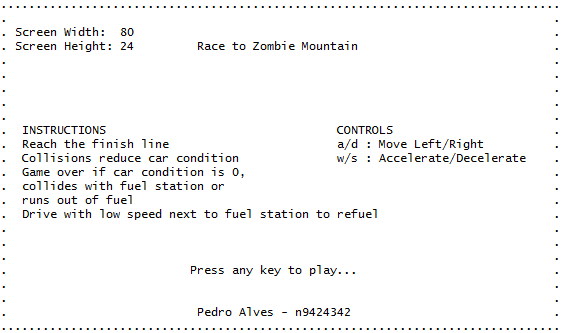
\includegraphics[width=0.95\textwidth]{images/border_80x24}
	\caption{The border with screen dimensions of 80x24}
	\label{fig:border_80x24} 
	\end{center}
\end{figure}
\subsubsection*{Screen: 126x31}
\begin{figure}[h]
	\begin{center}
	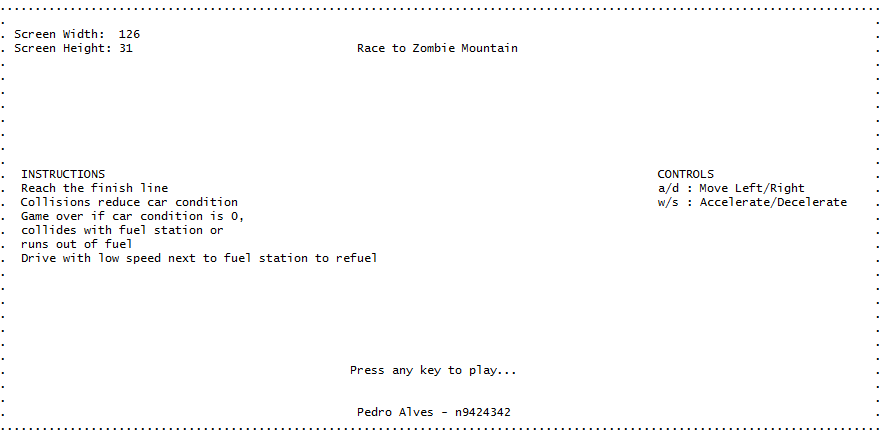
\includegraphics[width=1\textwidth]{images/border_126x31}
	\caption{The border with screen dimensions of 126x31}
	\label{fig:border_126x31} 
	\end{center}
\end{figure}
\subsubsection*{Screen: 190x50}
\begin{figure}[h]
	\begin{center}
	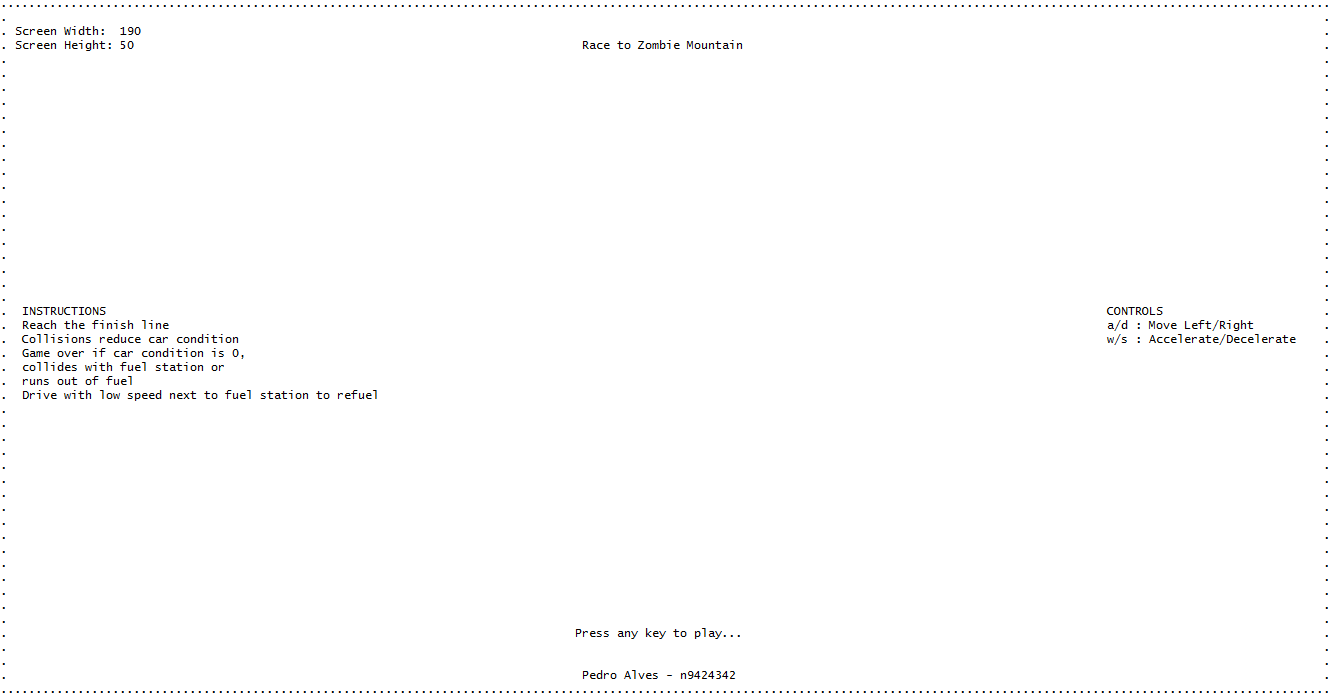
\includegraphics[width=0.745\textwidth]{images/border_190x50}
	\caption{The border with screen dimensions of 190x50}
	\label{fig:border_190x50} 
	\end{center}
\end{figure}

\clearpage
%----------------------------------------------------------------------------------------
%	DASHBOARD
%----------------------------------------------------------------------------------------
\section{Dashboard}
% Use 90x30 terminal size for examples
\clearpage

%----------------------------------------------------------------------------------------
%	RACE CAR
%----------------------------------------------------------------------------------------
\section{Race Car}

\clearpage

%----------------------------------------------------------------------------------------
%	HORIZONTAL MOVEMENT
%----------------------------------------------------------------------------------------
\section{Horizontal Movement}

\clearpage

%----------------------------------------------------------------------------------------
%	ACCELERATION AND SPEED
%----------------------------------------------------------------------------------------
\section{Acceleration and Speed}

\clearpage

%----------------------------------------------------------------------------------------
%	SCENERY AND OBSTACLES
%----------------------------------------------------------------------------------------
\section{Scenery and Obstacles}

\clearpage

%----------------------------------------------------------------------------------------
%	FUEL DEPOT
%----------------------------------------------------------------------------------------
\section{Fuel Depot}

\clearpage

%----------------------------------------------------------------------------------------
%	FUEL
%----------------------------------------------------------------------------------------
\section{Fuel}

\clearpage


%----------------------------------------------------------------------------------------
%	DISTANCE TRAVELLED
%----------------------------------------------------------------------------------------
\section{Distance Travelled}

\clearpage


%----------------------------------------------------------------------------------------
%	COLLISION
%----------------------------------------------------------------------------------------
\section{Collision}

\clearpage


%----------------------------------------------------------------------------------------
%	GAME OVER DIALOGUE
%----------------------------------------------------------------------------------------
\section{Game Over Dialogue}

\clearpage

%----------------------------------------------------------------------------------------
%	PARTB
%----------------------------------------------------------------------------------------
\section{Part B - Highscore Screen}

\clearpage



%----------------------------------------------------------------------------------------
%	REFERENCES
%----------------------------------------------------------------------------------------
\section{References}

\clearpage

\end{document}
